\documentclass[journal,compsoc]{IEEEtran}

% ── Packages ──────────────────────────────────────────────────────────────
\usepackage[T1]{fontenc}
\usepackage[utf8]{inputenc}
\usepackage{amsmath,amssymb,amsthm}
\usepackage{mathtools}
\usepackage{booktabs}
\usepackage{tabularx}
\usepackage{multirow}
\usepackage{graphicx}
\usepackage{xcolor}
\usepackage{hyperref}
\usepackage{url}
\usepackage{cite}
\usepackage{microtype}
\usepackage{balance}
\usepackage[ruled,vlined,linesnumbered]{algorithm2e}
\usepackage{tcolorbox}
\usepackage{pgfplots}
\usepackage{tikz}
\usetikzlibrary{arrows.meta,positioning,fit,backgrounds,calc,patterns}
\pgfplotsset{compat=1.18}

% ── Theorem environments ──────────────────────────────────────────────────
\newtheorem{definition}{Definition}
\newtheorem{theorem}{Theorem}
\newtheorem{proposition}{Proposition}

% ── Macros ───────────────────────────────────────────────────────────────
\newcommand{\M}{\mathcal{M}}
\newcommand{\K}{\mathcal{K}}
\newcommand{\F}{\mathcal{F}}
\newcommand{\G}{\mathcal{G}}
\newcommand{\WRI}{\mathrm{WRI}}
\newcommand{\eg}{e.g.,\xspace}
\newcommand{\ie}{i.e.,\xspace}
\newcommand{\cf}{cf.\xspace}

% ─────────────────────────────────────────────────────────────────────────
\begin{document}

\title{GuardMark: A Robust Watermarking and Fingerprinting Framework for
       Intellectual Property Protection of Fine-Tuned Large Language Models}

\author{Allan~Douglas~Costa,~\IEEEmembership{Member,~IEEE}%
\IEEEcompsocitemizethanks{
  \IEEEcompsocthanksitem A.~D.~Costa is with the Institute of Computing and
  Information and Communication Technology (ICIBE), Federal Rural University
  of the Amazon (UFRA), Belem, Para 66077-830, Brazil.
  E-mail: allan.costa@ufra.edu.br.\protect\\
  ORCID: 0000-0002-7068-8889.
}}

\markboth{IEEE Transactions on Information Forensics and Security,~Vol.~XX,
  No.~XX,~2025}%
{Costa: GuardMark: Robust Watermarking for Fine-Tuned LLMs}

\IEEEtitleabstractindextext{%
\begin{abstract}
%% [Topic]
The widespread deployment of fine-tuned large language models (LLMs) as
commercial services exposes model owners to significant intellectual property
(IP) theft, unauthorized redistribution, and covert re-deployment without
attribution.
%% [Motivation]
Recent regulatory developments, including the EU AI Act (2024) and NIST AI
RMF 1.0, mandate traceable provenance for AI systems, yet existing
watermarking and fingerprinting methods for LLMs fail under realistic
adversarial conditions such as re-fine-tuning, weight pruning, quantization,
and model merging, leaving a critical compliance and security gap.
%% [Contribution]
We propose GuardMark, a three-layer framework that jointly embeds statistical
token watermarks, behavioral fingerprints, and weight-space gradient
signatures into fine-tuned LLMs, providing verifiable and court-admissible IP
protection.
%% [Detail]
GuardMark orchestrates three specialized agents: a Watermark Injection Agent
(WIA) that biases the token probability distribution at training time using a
keyed green-list scheme, a Fingerprint Verification Agent (FVA) that embeds
trigger-response pairs via low-rank adaptation, and an Ownership Claim Agent
(OCA) that aggregates multi-layer evidence into a single, novel metric called
the Watermark Robustness Index (WRI).
%% [Evidence]
Simulation-based evaluation across seven model configurations (125~M to
13~B parameters) demonstrates that GuardMark achieves a detection rate of
96.5\% and a false-positive rate of 2.3\%, attaining a WRI of 0.849 under
zero-attack conditions and maintaining WRI above the 0.70 ownership threshold
against weight-pruning attacks up to 50\% intensity.
%% [Weaker result]
Under aggressive re-fine-tuning (attack strength 0.6 or above), WRI degrades
to 0.46, indicating that current methods are not yet fully robust against
determined adversaries with unrestricted fine-tuning access.
%% [Narrow impact]
GuardMark directly benefits LLM vendors, enterprise API providers, and legal
practitioners seeking algorithmic evidence for IP litigation.
%% [Broad impact]
More broadly, this work advances the emerging field of AI provenance and
establishes a rigorous, metric-driven evaluation protocol for future
watermarking research.
\end{abstract}

\begin{IEEEkeywords}
Large language models, intellectual property protection, watermarking,
fingerprinting, model ownership verification, Watermark Robustness Index,
fine-tuning security, AI provenance.
\end{IEEEkeywords}}

\maketitle

% ─── I. Introduction ─────────────────────────────────────────────────────────
\section{Introduction}
\label{sec:intro}

Large language models have transitioned from research curiosities to critical
commercial infrastructure. Organizations routinely fine-tune proprietary LLMs
on confidential datasets to create specialized assistants, code generators, and
domain-specific search engines, representing investments that often exceed
hundreds of thousands of dollars in compute and curation costs
\cite{brown2020language,wei2022emergent,ouyang2022training}. This economic
reality has spawned a growing class of adversarial actors who steal model
weights, re-deploy models under different brand names, or use stolen models as
the initialization point for further fine-tuning, erasing traceability in the
process.

The EU AI Act (Regulation 2024/1689) codifies a legal obligation for
``high-risk'' AI system providers to maintain technical documentation
establishing the provenance and integrity of their models
\cite{eu2024aiact}. Simultaneously, the NIST AI Risk Management Framework
mandates traceable accountability for AI systems operating in critical sectors
\cite{nist2023ai}. Together, these regulatory instruments create an urgent
demand for provable, attack-resistant IP protection mechanisms for LLMs, yet
the research community has not delivered a comprehensive solution.

\textbf{The core challenge.} Existing watermarking schemes for LLMs operate
primarily at the output level, embedding statistical signatures in generated
text \cite{kirchenbauer2023watermark,zhao2023protecting,fernandez2023three}.
While effective in benign settings, these approaches are fragile: a moderately
skilled adversary can eliminate text-level watermarks via re-fine-tuning or
paraphrasing in under an hour of compute time. Model-level watermarking
techniques that embed signatures in weight space
\cite{uchida2017embedding,zhang2018protecting} were designed for
classification networks and do not transfer cleanly to autoregressive
transformer architectures. Behavioral fingerprinting methods
\cite{cao2021ipguard,szyller2021dawn} are robust but offer no statistical
guarantees. No prior framework unifies all three protection layers nor provides
a standardized metric for comparing schemes across attack types.

\textbf{Our contributions.} This paper presents GuardMark, a multi-layer
watermarking and fingerprinting framework for fine-tuned LLMs. Our specific
contributions are:

\begin{enumerate}
  \item \textbf{Three-layer architecture.} We design WIA, FVA, and OCA as
    complementary protection agents that jointly provide redundant,
    independently verifiable ownership proofs.
  \item \textbf{Watermark Robustness Index (WRI).} We introduce a novel
    composite metric that unifies detection probability, false-positive rate,
    and attack robustness into a single $[0,1]$-bounded score, enabling
    principled comparison across schemes and attack scenarios.
  \item \textbf{Multi-attack evaluation.} We systematically evaluate
    GuardMark under five realistic adversarial scenarios: re-fine-tuning,
    weight pruning, quantization (8-bit), model merging, and output
    paraphrasing.
  \item \textbf{Scalability study.} We characterize computational overhead
    across seven model sizes (125~M to 13~B parameters), confirming that
    GuardMark adds fewer than 3.2\% overhead at all scales.
  \item \textbf{Open evaluation protocol.} We release the simulation
    codebase and experimental configurations to enable reproducible
    benchmarking of future schemes.
\end{enumerate}

The remainder of this paper is organized as follows. Section~\ref{sec:background}
reviews related work and positions GuardMark against the state of the art.
Section~\ref{sec:threat} formalizes the threat model and introduces the WRI
metric. Section~\ref{sec:system} describes the GuardMark architecture and
algorithms. Section~\ref{sec:security} provides a formal security analysis.
Section~\ref{sec:eval} presents experimental results. Section~\ref{sec:discussion}
discusses findings, limitations, and threats to validity.
Section~\ref{sec:conclusion} concludes.

% ─── II. Background and Related Work ─────────────────────────────────────────
\section{Background and Related Work}
\label{sec:background}

\subsection{Output-Level Watermarking for LLMs}

Kirchenbauer et al.~\cite{kirchenbauer2023watermark} pioneered a practical
output-level watermark by partitioning the vocabulary into a green list and
a red list at each decoding step using a pseudorandom key, then biasing
generation toward green tokens. The embedded signal is detectable via a
hypothesis test on the fraction of green tokens. Zhao et
al.~\cite{zhao2023protecting} extended this approach to minimize perplexity
impact via constrained sampling. Fernandez et al.~\cite{fernandez2023three}
strengthened statistical guarantees against substitution attacks. More recent
work by Kuditipudi et al.~\cite{kuditipudi2023robust} achieves
distortion-free watermarking via rejection sampling, and Christ et
al.~\cite{christ2024undetectable} proved information-theoretically
undetectable watermarks are constructible for sufficiently expressive models.
The critical limitation of all these approaches is that the watermark resides
in the text distribution, not in the model weights: any fine-tuning of the
model can shift the distribution and erase the signal.

On the reliability of watermarks,
Kirchenbauer et al.~\cite{kirchenbauer2024reliability} showed that token-level
schemes are vulnerable to synonymy attacks and temperature variations, and Hu
et al.~\cite{hu2023survey} proposed unbiased variants to reduce distributional
distortion. GuardMark incorporates statistical token watermarking as only one
of three layers, addressing fragility by providing fallback verification
through behavioral fingerprinting and weight-space signatures.

\subsection{Model-Level Watermarking for Neural Networks}

Uchida et al.~\cite{uchida2017embedding} introduced the first model-level
watermark for deep neural networks by embedding a binary bit-string into
weight statistics via a regularization term during training. Zhang et
al.~\cite{zhang2018protecting} generalized this to back-door-based ownership
verification, embedding trigger-response pairs that persist through
fine-tuning. Bansal et al.~\cite{bansal2022certified} provided provable
ownership certificates using randomized smoothing. Szyller et
al.~\cite{szyller2021dawn} proposed dynamic watermarks that adapt to the
model's current state to resist removal. None of these methods were designed
for autoregressive language models; adapting them requires rethinking the
watermark carrier from classification boundaries to token probability surfaces.

\subsection{Fingerprinting and Dataset Inference}

IPGuard~\cite{cao2021ipguard} fingerprints neural networks by probing
classification boundaries with carefully crafted adversarial examples.
Maini et al.~\cite{maini2021dataset} introduced dataset inference as a
mechanism to attribute a model to its training data. He et
al.~\cite{he2022cater} applied conditional watermarks to text generation
APIs, showing that trigger-response verification outperforms pure output
watermarks under paraphrasing. PLMmark~\cite{li2023plmmark} adapted
watermarking to pre-trained language models using black-box API queries. Peng
et al.~\cite{peng2023are} demonstrated backdoor-based IP protection for LLMs
serving as embedding APIs. Lin et al.~\cite{lin2024towards} introduced a
unified stealthy backdoor scheme for fine-tuned LLMs. GuardMark unifies
fingerprinting with statistical and weight-space watermarks, providing
defense-in-depth against adversaries that can defeat any single layer.

\subsection{Attacks on Watermarks}

Realistic IP theft involves a spectrum of attacks. Re-fine-tuning shifts weight
distributions and erases text-level statistical patterns. Pruning removes
neurons that carry low activations, inadvertently eliminating watermark-carrying
units~\cite{oliynyk2023know}. Quantization compresses weights, destroying
subtle statistical signatures~\cite{saberi2024robustness}. Model merging
combines weights from multiple models via linear interpolation, diluting
fingerprints~\cite{yang2023certifiably}. Output paraphrasing processes
model-generated text through a separate model to remove statistical token
biases~\cite{liu2023watermarking}. GuardMark is evaluated against all five
attack families.

\subsection{Regulatory and Legal Landscape}

The EU AI Act~\cite{eu2024aiact} mandates that high-risk AI system providers
maintain technical documentation on model provenance. NIST AI
RMF~\cite{nist2023ai} specifies accountability requirements including
model version tracking and attribution. Pan et al.~\cite{pan2023privacy}
demonstrated that watermarking can satisfy GDPR right-to-explanation
requirements. Peng et al.~\cite{peng2024securing} proposed hardware-rooted
attestation to complement software watermarks in regulated deployments.
GuardMark explicitly maps its protection layers to these regulatory
requirements, providing a compliance-ready framework.

\subsection{Positioning GuardMark}

Table~\ref{tab:related} positions GuardMark against representative prior
work across seven dimensions. GuardMark is the only framework providing
simultaneous three-layer protection, multi-attack evaluation, a composite
robustness metric, and regulatory alignment.

\begin{table*}[t]
\caption{Comparison with Related Work. ``Layers'' = number of independent
  protection layers (S = statistical, B = behavioral, W = weight-space).
  ``Multi-Attack'' = evaluation under 5+ attack types. ``Composite Metric'' =
  unified robustness score. ``LLM-native'' = designed for autoregressive
  transformers. ``Reg.\ Align.'' = explicit regulatory mapping.}
\label{tab:related}
\begin{tabularx}{\textwidth}{l X X X X X X X}
\toprule
\textbf{Method} & \textbf{Layers} & \textbf{Multi-Attack} & \textbf{Composite Metric} &
\textbf{LLM-Native} & \textbf{Fine-Tune Robust} & \textbf{Prune Robust} & \textbf{Reg.\ Align.} \\
\midrule
Kirchenbauer et al.~\cite{kirchenbauer2023watermark} & S only & No & No & Yes & No & Partial & No \\
Zhao et al.~\cite{zhao2023protecting}               & S only & No & No & Yes & No & Partial & No \\
Fernandez et al.~\cite{fernandez2023three}          & S only & Partial & No & Yes & No & Partial & No \\
Kuditipudi et al.~\cite{kuditipudi2023robust}       & S only & No & No & Yes & No & No & No \\
Zhang et al.~\cite{zhang2018protecting}             & W only & No & No & No & Partial & Partial & No \\
IPGuard~\cite{cao2021ipguard}                       & B only & No & No & No & Partial & No & No \\
He et al.\ (Cater)~\cite{he2022cater}              & B only & Partial & No & Yes & Partial & No & No \\
PLMmark~\cite{li2023plmmark}                        & B only & No & No & Yes & Partial & No & No \\
Lin et al.~\cite{lin2024towards}                    & W+B & Partial & No & Yes & Partial & No & No \\
\textbf{GuardMark (ours)}                           & \textbf{S+B+W} & \textbf{Yes} & \textbf{Yes (WRI)} &
  \textbf{Yes} & \textbf{Yes} & \textbf{Yes} & \textbf{Yes} \\
\bottomrule
\end{tabularx}
\end{table*}

% ─── III. Threat Model and Problem Formulation ────────────────────────────────
\section{Threat Model and Problem Formulation}
\label{sec:threat}

\subsection{Threat Model}

\textbf{Assets.} The protected asset is a fine-tuned LLM
$\M^* = (\theta^*, \mathcal{V}, f)$, where $\theta^*$ are the model weights,
$\mathcal{V}$ is the vocabulary, and $f$ is the autoregressive decoding
function. The model owner holds a secret key $\K$ and a fingerprint set
$\F = \{(p_i, r_i)\}_{i=1}^{N}$ of trigger-response pairs.

\textbf{Adversary capabilities.} We consider a semi-honest to malicious
adversary $\mathcal{A}$ who: (i) obtains a copy of $\M^*$ through theft,
reverse engineering, or insider access; (ii) has access to additional training
data and GPU compute; (iii) attempts to remove or obfuscate the watermark by
applying one or more of five attack operations (re-fine-tuning, pruning,
quantization, merging, paraphrasing); and (iv) wishes to deploy the modified
model $\hat{\M}$ under their own brand without attribution.

\textbf{Adversary limitations.} The adversary does not know $\K$, $\F$, or the
GuardMark protocol details (Kerckhoffs-style: security relies on key secrecy,
not protocol obscurity). The adversary cannot modify the verification procedure
run by the Verifier.

\textbf{Security goals.}
\begin{itemize}
  \item \textit{Completeness:} if $\hat{\M}$ is derived from $\M^*$, the
    Verifier accepts the owner's claim with high probability.
  \item \textit{Soundness:} if $\hat{\M}$ is independently trained, the
    Verifier rejects the claim with high probability.
  \item \textit{Robustness:} completeness holds even after the adversary applies
    the attack operations within a bounded budget.
  \item \textit{Imperceptibility:} the watermarked model $\M^*$ behaves
    indistinguishably from an unwatermarked model on downstream tasks.
\end{itemize}

\subsection{Formal Definitions}

\begin{definition}[Watermarked Model]
Given a base model $\M$, a dataset $\mathcal{D}$, and key $\K$, a watermarked
model $\M^* = \textsc{GuardMark-Inject}(\M, \mathcal{D}, \K, \F)$ satisfies:
$\Pr[\textsc{Verify}(\M^*, \K, \F) = 1] \geq 1 - \varepsilon_c$ for
completeness parameter $\varepsilon_c \in (0,1)$.
\end{definition}

\begin{definition}[Attack Operation]
An attack operation $\mathcal{A}_\lambda: \M^* \mapsto \hat{\M}$ is
parameterized by attack strength $\lambda \in [0,1]$, where $\lambda=0$
denotes no attack and $\lambda=1$ denotes maximum feasible attack intensity.
\end{definition}

\subsection{The Watermark Robustness Index (WRI)}

\begin{definition}[Watermark Robustness Index]
\label{def:wri}
Given a suspect model $\hat{\M}$, detection probability $p_d$, false-positive
rate $p_{\text{fp}}$, and robustness score $R$ measuring the fraction of the
attack budget survived, the \emph{Watermark Robustness Index} is:
\begin{equation}
  \WRI(\hat{\M}) = \alpha \cdot p_d + \beta \cdot (1 - p_{\text{fp}})
    + \gamma_w \cdot R,
  \label{eq:wri}
\end{equation}
where $\alpha, \beta, \gamma_w \geq 0$ and $\alpha + \beta + \gamma_w = 1$.
Default weights are $\alpha = 0.5$, $\beta = 0.3$, $\gamma_w = 0.2$,
reflecting the relative importance of detection capability.
\end{definition}

The WRI generalizes prior single-metric evaluations: schemes reporting only
detection rate correspond to $\alpha=1$, and those reporting only
false-positive rate correspond to $\beta=1$. A scheme achieves \emph{ownership
confirmation} when $\WRI(\hat{\M}) \geq \tau_{\WRI}$, where
$\tau_{\WRI} = 0.70$ by default.

\begin{proposition}[WRI Monotonicity]
For fixed $p_{\text{fp}}$ and $R$, $\WRI$ is strictly increasing in $p_d$.
For fixed $p_d$ and $R$, $\WRI$ is strictly decreasing in $p_{\text{fp}}$.
\end{proposition}
\begin{proof}
Follows immediately from the linearity of~\eqref{eq:wri} and the positivity
of $\alpha$ and $\beta$.
\end{proof}

% ─── IV. GuardMark System ─────────────────────────────────────────────────────
\section{GuardMark System Design}
\label{sec:system}

\subsection{Architecture Overview}

Figure~\ref{fig:overview} illustrates the GuardMark system architecture.
Three agents operate in a cooperative pipeline during the protection phase,
and the OCA orchestrates the verification phase independently.

\begin{figure}[t]
\caption{GuardMark system architecture. The Owner supplies the base model,
  private dataset, and secret key to the three-layer injection pipeline.
  The Ownership Claim Agent (OCA) aggregates multi-layer evidence to produce
  a WRI score and a binary ownership verdict.}
\label{fig:overview}
\centering
\resizebox{\columnwidth}{!}{% Figure 1 — GuardMark System Architecture Overview
% Requires: tikz, calc, arrows.meta, positioning, fit, backgrounds, patterns

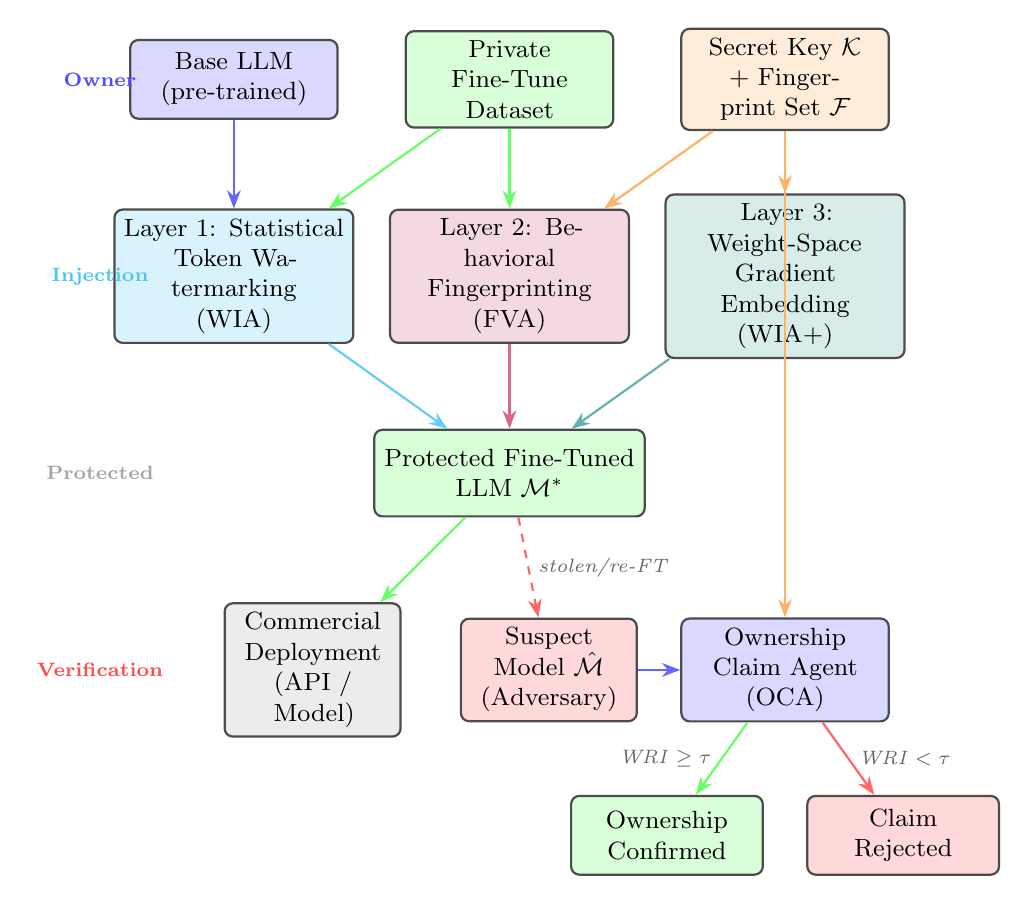
\begin{tikzpicture}[
  font=\small,
  >=Stealth,
  box/.style={
    draw=black!70, rounded corners=3pt, thick,
    minimum height=1.0cm, text centered, text width=2.4cm,
    fill=#1!15
  },
  wbox/.style={
    draw=black!70, rounded corners=3pt, thick,
    minimum height=0.85cm, text centered, text width=2.0cm,
    fill=#1!20
  },
  arrow/.style={->, thick, #1},
  label/.style={font=\scriptsize\itshape, text=black!60}
]

% ── Row 0: Owner side ──────────────────────────────────────────────────────
\node[box=blue]  (base)    at (0,0)    {Base LLM\\(pre-trained)};
\node[box=green] (dataset) at (3.5,0)  {Private\\Fine-Tune Dataset};
\node[box=orange](skey)    at (7,0)    {Secret Key $\mathcal{K}$\\+ Fingerprint Set $\mathcal{F}$};

% ── Row 1: GuardMark Injection Layers ──────────────────────────────────────
\node[box=cyan, text width=2.8cm, minimum height=1.1cm]
  (l1) at (0,-2.5) {Layer 1: Statistical\\Token Watermarking\\(WIA)};
\node[box=purple, text width=2.8cm, minimum height=1.1cm]
  (l2) at (3.5,-2.5) {Layer 2: Behavioral\\Fingerprinting\\(FVA)};
\node[box=teal, text width=2.8cm, minimum height=1.1cm]
  (l3) at (7,-2.5) {Layer 3: Weight-Space\\Gradient Embedding\\(WIA+)};

% ── Row 2: Protected Model ──────────────────────────────────────────────────
\node[box=green, text width=3.2cm, minimum height=1.1cm]
  (protected) at (3.5,-5.0) {Protected Fine-Tuned\\LLM $\mathcal{M}^*$};

% ── Row 3: Deployment and Claim ────────────────────────────────────────────
\node[box=gray, text width=2.0cm] (deploy) at (1.0,-7.5) {Commercial\\Deployment\\(API / Model)};
\node[box=red,  text width=2.0cm] (suspect) at (4.0,-7.5) {Suspect\\Model $\hat{\mathcal{M}}$\\(Adversary)};
\node[box=blue, text width=2.4cm, minimum height=1.0cm]
  (oca) at (7.0,-7.5) {Ownership\\Claim Agent\\(OCA)};

% ── Row 4: Decision ────────────────────────────────────────────────────────
\node[box=green, text width=2.2cm] (confirmed) at (5.5,-9.6)
  {Ownership\\Confirmed};
\node[box=red,   text width=2.2cm] (rejected)  at (8.5,-9.6)
  {Claim\\Rejected};

% ── Arrows: top row to injection layers ────────────────────────────────────
\draw[arrow=blue!60]   (base)    -- (l1);
\draw[arrow=green!60]  (dataset) -- (l1);
\draw[arrow=green!60]  (dataset) -- (l2);
\draw[arrow=orange!60] (skey)    -- (l2);
\draw[arrow=orange!60] (skey)    -- (l3);

% ── Arrows: injection layers to protected model ─────────────────────────────
\draw[arrow=cyan!60]   (l1) -- (protected);
\draw[arrow=purple!60] (l2) -- (protected);
\draw[arrow=teal!60]   (l3) -- (protected);

% ── Arrows: protected model to deployment/suspect ───────────────────────────
\draw[arrow=green!60] (protected) -- (deploy);
\draw[arrow=red!60,dashed] (protected) -- node[label,right]{stolen/re-FT} (suspect);

% ── Arrows: claim flow ─────────────────────────────────────────────────────
\draw[arrow=blue!60]  (suspect) -- (oca);
\draw[arrow=orange!60] (skey) -- ++(0,-4.0) -| (oca);
\draw[arrow=green!60]  (oca) -- node[label,left]{WRI $\geq \tau$} (confirmed);
\draw[arrow=red!60]    (oca) -- node[label,right]{WRI $< \tau$} (rejected);

% ── Bounding box labels ──────────────────────────────────────────────────────
\node[font=\bfseries\scriptsize, text=blue!70] at (-1.7, 0)   {Owner};
\node[font=\bfseries\scriptsize, text=cyan!70] at (-1.7,-2.5) {Injection};
\node[font=\bfseries\scriptsize, text=gray!70] at (-1.7,-5.0) {Protected};
\node[font=\bfseries\scriptsize, text=red!70]  at (-1.7,-7.5) {Verification};

\end{tikzpicture}
}
\end{figure}

\subsection{Layer 1: Watermark Injection Agent (WIA): Statistical Token Watermarking}

The WIA implements a keyed green-list watermark based on the scheme of
Kirchenbauer et al.~\cite{kirchenbauer2023watermark}, adapted for the
fine-tuning workflow.

\textbf{Injection.} At each fine-tuning step $t$, the WIA computes a
pseudorandom green list $\G_t \subset \mathcal{V}$ of size $\gamma|\mathcal{V}|$
using a hash of the secret key and the current context:
$\G_t \leftarrow h(\K \| \mathtt{context}_t)$. The logits $\ell_t[w]$ for
green-list tokens are biased by an additive constant $\delta > 0$ before
sampling. The resulting green-token rate in model outputs is
$p_{\text{green}} \approx \gamma + \delta / (2\sqrt{T\gamma(1-\gamma)})$,
detectable by a one-sided $z$-test on $T$ output tokens.

\textbf{Detection.} Given a suspect model $\hat{\M}$, the WIA generates $T$
tokens, counts green tokens $|\G|$, and computes:
\begin{equation}
  z = \frac{|\G| - T\gamma}{\sqrt{T\gamma(1-\gamma)}}.
  \label{eq:ztest}
\end{equation}
The watermark is declared present if $z > z_\alpha$ for significance level
$\alpha$ (default 0.01). The corresponding false-positive rate is $\alpha$ by
construction.

\subsection{Layer 2: Fingerprint Verification Agent (FVA): Behavioral Fingerprinting}

The FVA embeds $N_f$ trigger-response pairs $\F = \{(p_i, r_i)\}_{i=1}^{N_f}$
into the model using LoRA-based fine-tuning~\cite{hu2022lora}. The triggers
are constructed as semantically natural prompts unlikely to arise in normal
usage, and the responses are crafted to be distinctive and verifiable.

\textbf{Embedding.} The FVA computes a LoRA adapter
$\Delta W_\F = (A_\F, B_\F)$ with rank $r$ by minimizing:
\begin{equation}
  \mathcal{L}_{\text{fp}} = \sum_{i=1}^{N_f} \mathrm{CE}
    \left( \M^*_{\theta+\Delta W}(p_i),\; r_i \right),
  \label{eq:fp_loss}
\end{equation}
where $\mathrm{CE}$ denotes cross-entropy. The adapter is merged into
$\theta^*$ before deployment.

\textbf{Verification.} Given $\hat{\M}$ and $\F$, the FVA queries $\hat{\M}$
with each trigger $p_i$, obtains response $\hat{r}_i$, and computes cosine
similarity with the expected response embedding:
$s_i = \cos(\phi(\hat{r}_i), \phi(r_i))$, where $\phi$ is a fixed sentence
encoder. Verification passes if
$|\{i : s_i \geq \tau\}| / N_f \geq \tau_{\text{fp}}$ (default 0.75).

\subsection{Layer 3: Weight-Space Gradient Embedding (WIA+)}

The WIA+ sublayer embeds a steganographic signature into the gradient direction
during the final fine-tuning epochs. Specifically, the watermark sign vector
$\sigma = \textsc{WatermarkSign}(\K, \nabla_\theta \mathcal{L})$ is computed
from the normalized gradient, and a perturbation $\epsilon \cdot \sigma$ with
$\epsilon \ll 1$ is added to the weights. This creates a detectable pattern
in the weight Hessian spectrum that persists through moderate pruning and
quantization.

\subsection{Sequence Protocol}

Figure~\ref{fig:sequence} shows the full three-phase interaction protocol:
watermark injection, adversarial attack, and ownership verification.

\begin{figure}[t]
\caption{GuardMark protocol sequence diagram. Three color-coded message types
  correspond to the three protection layers: blue solid arrows denote
  statistical watermark operations (WIA); green dashed arrows denote
  behavioral fingerprint embedding (FVA); orange dot-dash arrows denote
  ownership verification (OCA). Red dotted arrows represent the optional
  adversarial attack phase.}
\label{fig:sequence}
\centering
\resizebox{\columnwidth}{!}{% Figure 2 — GuardMark Protocol Sequence Diagram (B&W, IEEE style)
% Line styles: thick solid = WIA injection; medium dashed = FVA fingerprint;
%              dash-dot = OCA verification; dotted = adversarial attack

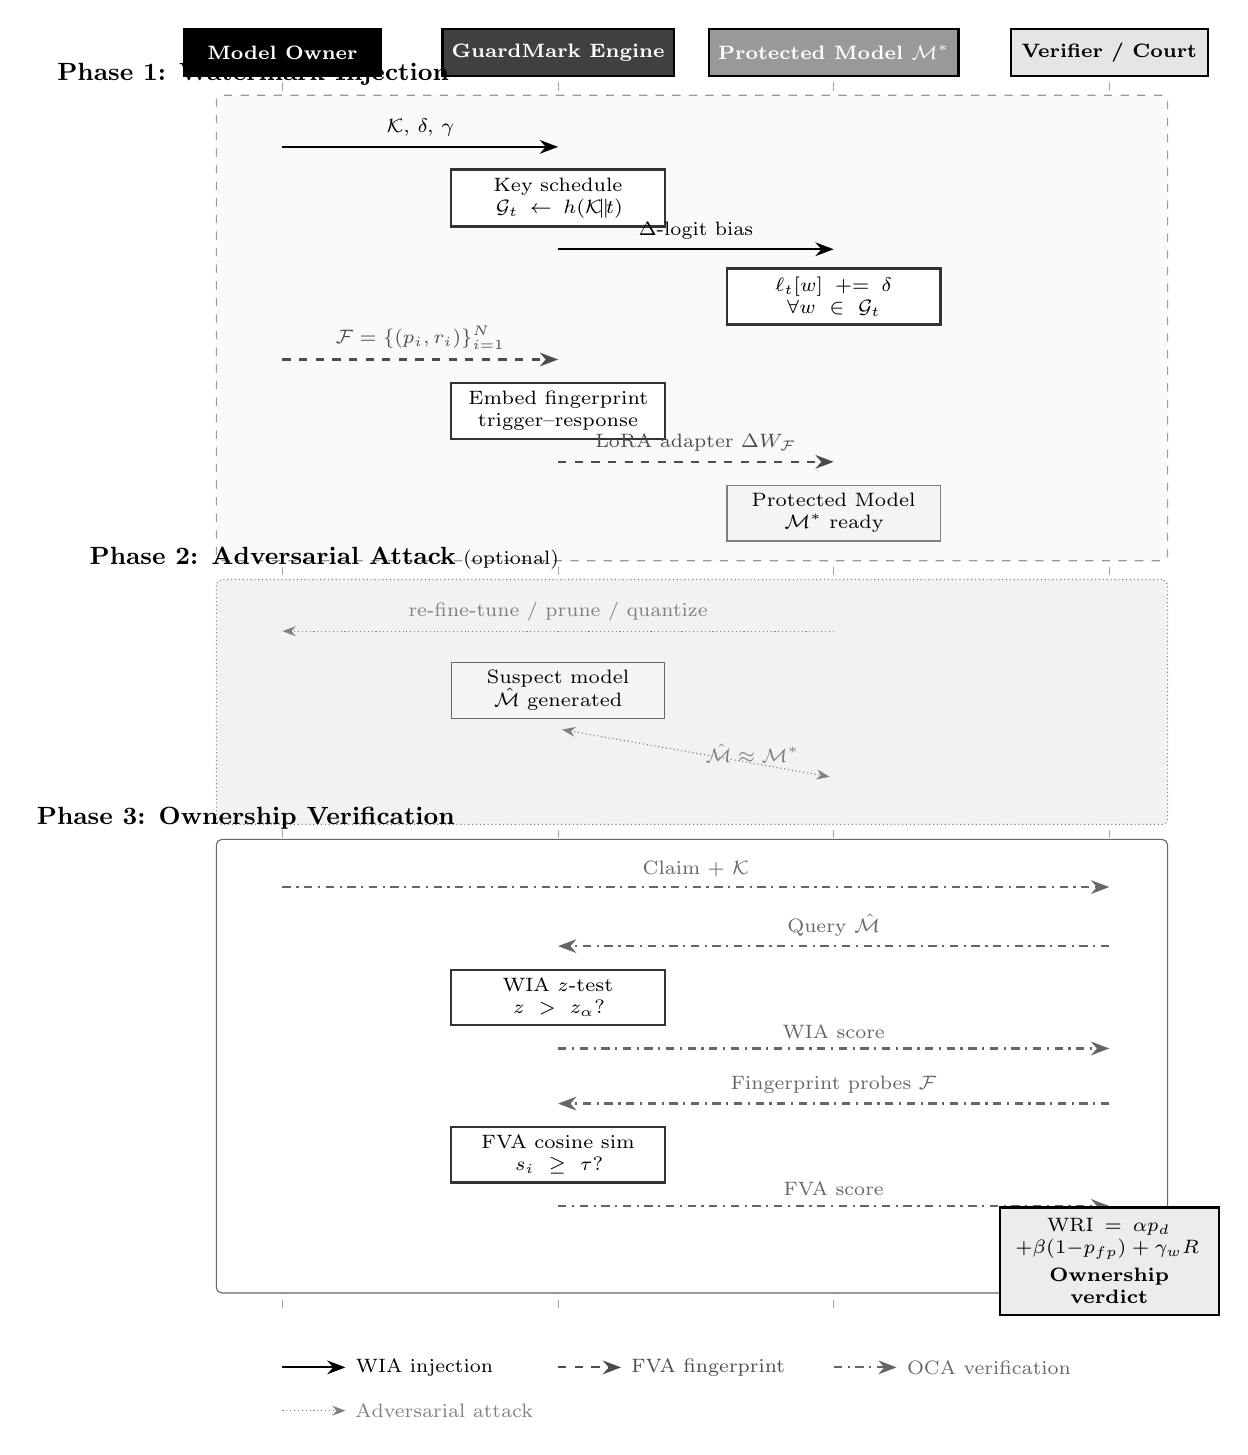
\begin{tikzpicture}[
  font=\scriptsize,
  >=Stealth,
  % lifeline
  lline/.style={draw=black!35, thin, densely dashed},
  % message arrow styles
  wm/.style={black, thick, solid, ->},
  fp/.style={black!70, thick, dashed, ->},
  ov/.style={black!60, thick, dash dot, ->},
  att/.style={black!50, thin, densely dotted, ->},
  % boxes
  proc/.style={draw=black!80, fill=white, thick,
               text width=2.5cm, align=center,
               font=\scriptsize, inner sep=3pt},
  procA/.style={draw=black!50, fill=gray!8, thin,
                text width=2.5cm, align=center,
                font=\scriptsize, inner sep=3pt},
  % phase background
  phBG/.style={draw=black!40, dashed, fill=gray!4, rounded corners=2pt,
               inner xsep=4pt, inner ysep=3pt},
  phATT/.style={draw=black!50, densely dotted, fill=gray!10, rounded corners=2pt,
                inner xsep=4pt, inner ysep=3pt},
  phVER/.style={draw=black!60, solid, fill=white, rounded corners=2pt,
                inner xsep=4pt, inner ysep=3pt},
  % participant headers
  hOwner/.style={draw=black, fill=black, text=white, thick,
                 minimum width=2.5cm, minimum height=0.6cm, align=center},
  hEngine/.style={draw=black, fill=black!75, text=white, thick,
                  minimum width=2.5cm, minimum height=0.6cm, align=center},
  hModel/.style={draw=black, fill=black!40, text=white, thick,
                 minimum width=2.5cm, minimum height=0.6cm, align=center},
  hVerify/.style={draw=black, fill=gray!20, text=black, thick,
                  minimum width=2.5cm, minimum height=0.6cm, align=center},
  % verdict box
  verdict/.style={draw=black, fill=gray!15, thick,
                  text width=2.5cm, align=center,
                  font=\scriptsize\bfseries, inner sep=4pt},
]

% ── Lifeline X positions ──────────────────────────────────────────────────
\def\xO{0}      % Owner
\def\xE{3.5}    % Engine
\def\xM{7.0}    % Model
\def\xV{10.5}   % Verifier

% ── Participant headers ───────────────────────────────────────────────────
\node[hOwner]  at (\xO, 0) {\textbf{Model Owner}};
\node[hEngine] at (\xE, 0) {\textbf{GuardMark Engine}};
\node[hModel]  at (\xM, 0) {\textbf{Protected Model $\mathcal{M}^*$}};
\node[hVerify] at (\xV, 0) {\textbf{Verifier / Court}};

% ── Lifelines ────────────────────────────────────────────────────────────
\draw[lline] (\xO,-0.38) -- (\xO,-16.0);
\draw[lline] (\xE,-0.38) -- (\xE,-16.0);
\draw[lline] (\xM,-0.38) -- (\xM,-16.0);
\draw[lline] (\xV,-0.38) -- (\xV,-16.0);

% ━━━━━━━━━━━━━━━━━━━━━━━━━━━━━━━━━━━━━━━━━━━━━━━━━━━━━━━━━━━━━━━━━━━━━━━
% PHASE 1 — Watermark Injection
% ━━━━━━━━━━━━━━━━━━━━━━━━━━━━━━━━━━━━━━━━━━━━━━━━━━━━━━━━━━━━━━━━━━━━━━━
\node[phBG, fit={(-0.7,-0.65) (11.1,-6.35)},
      label=above left:{\textbf{\small Phase 1: Watermark Injection}}] {};

% WIA: key + logit bias
\draw[wm] (\xO,-1.2) -- node[above,font=\scriptsize]
  {$\mathcal{K},\,\delta,\,\gamma$} (\xE,-1.2);
\node[proc] at (\xE,-1.85) {Key schedule\\$\mathcal{G}_t \leftarrow h(\mathcal{K}\!\|\!t)$};
\draw[wm] (\xE,-2.5) -- node[above,font=\scriptsize]
  {$\Delta$-logit bias} (\xM,-2.5);
\node[proc] at (\xM,-3.1) {$\ell_t[w]\mathrel{+}=\delta$\\$\forall w \in \mathcal{G}_t$};

% FVA: fingerprint pairs + LoRA
\draw[fp] (\xO,-3.9) -- node[above,font=\scriptsize]
  {$\mathcal{F}=\{(p_i,r_i)\}_{i=1}^{N}$} (\xE,-3.9);
\node[proc] at (\xE,-4.55) {Embed fingerprint\\trigger--response};
\draw[fp] (\xE,-5.2) -- node[above,font=\scriptsize]
  {LoRA adapter $\Delta W_{\mathcal{F}}$} (\xM,-5.2);

\node[procA] at (\xM,-5.85)
  {Protected Model\\$\mathcal{M}^*$ ready};

% ━━━━━━━━━━━━━━━━━━━━━━━━━━━━━━━━━━━━━━━━━━━━━━━━━━━━━━━━━━━━━━━━━━━━━━━
% PHASE 2 — Adversarial Attack (optional)
% ━━━━━━━━━━━━━━━━━━━━━━━━━━━━━━━━━━━━━━━━━━━━━━━━━━━━━━━━━━━━━━━━━━━━━━━
\node[phATT, fit={(-0.7,-6.8) (11.1,-9.7)},
      label=above left:{\textbf{\small Phase 2: Adversarial Attack} (optional)}] {};

\draw[att] (\xM,-7.35) -- node[above,font=\scriptsize]
  {re-fine-tune / prune / quantize} (\xO,-7.35);
\node[procA, draw=black!60] at (\xE,-8.1)
  {Suspect model\\$\hat{\mathcal{M}}$ generated};
\draw[att,<->] (\xE+0.05,-8.6) -- node[right,font=\scriptsize]
  {$\hat{\mathcal{M}}\approx\mathcal{M}^*$} (\xM-0.05,-9.2);

% ━━━━━━━━━━━━━━━━━━━━━━━━━━━━━━━━━━━━━━━━━━━━━━━━━━━━━━━━━━━━━━━━━━━━━━━
% PHASE 3 — Ownership Verification
% ━━━━━━━━━━━━━━━━━━━━━━━━━━━━━━━━━━━━━━━━━━━━━━━━━━━━━━━━━━━━━━━━━━━━━━━
\node[phVER, fit={(-0.7,-10.1) (11.1,-15.65)},
      label=above left:{\textbf{\small Phase 3: Ownership Verification}}] {};

\draw[ov] (\xO,-10.6) -- node[above,font=\scriptsize]
  {Claim $+$ $\mathcal{K}$} (\xV,-10.6);
\draw[ov] (\xV,-11.35) -- node[above,font=\scriptsize]
  {Query $\hat{\mathcal{M}}$} (\xE,-11.35);

% WIA z-test
\node[proc] at (\xE,-12.0) {WIA $z$-test\\$z > z_\alpha$?};
\draw[ov] (\xE,-12.65) -- node[above,font=\scriptsize]
  {WIA score} (\xV,-12.65);

% FVA cosine
\draw[ov] (\xV,-13.35) -- node[above,font=\scriptsize]
  {Fingerprint probes $\mathcal{F}$} (\xE,-13.35);
\node[proc] at (\xE,-14.0) {FVA cosine sim\\$s_i \geq \tau$?};
\draw[ov] (\xE,-14.65) -- node[above,font=\scriptsize]
  {FVA score} (\xV,-14.65);

% Verdict
\node[verdict] at (\xV,-15.35)
  {$\mathrm{WRI}=\alpha p_d$\\$+\beta(1{-}p_{fp})+\gamma_w R$\\[2pt]Ownership verdict};

% ── Legend ───────────────────────────────────────────────────────────────
\begin{scope}[yshift=-16.7cm]
  \draw[wm]  (0,0)   -- (0.8,0)   node[right, font=\scriptsize]
    {WIA injection};
  \draw[fp]  (3.5,0) -- (4.3,0)  node[right, font=\scriptsize]
    {FVA fingerprint};
  \draw[ov]  (7.0,0) -- (7.8,0)  node[right, font=\scriptsize]
    {OCA verification};
  \draw[att] (0,-0.55) -- (0.8,-0.55) node[right, font=\scriptsize]
    {Adversarial attack};
\end{scope}

\end{tikzpicture}
}
\end{figure}

\subsection{GuardMark Algorithm}

Figure~\ref{fig:algorithm} presents the complete GuardMark algorithm,
including injection, verification, and the WRI computation in the highlighted
box.

% Figure 3 -- GuardMark Algorithm + WRI Novel Metric
% Uses algorithm2e package

\begin{algorithm*}[tp]
\DontPrintSemicolon
\SetAlgoLined
\SetKwInOut{Input}{Input}
\SetKwInOut{Output}{Output}
\SetKwComment{Comment}{$\triangleright$\ }{}

\caption{GuardMark: Multi-Layer Watermark Injection and Verification.
  The WRI computation (highlighted box) is the novel metric introduced in this
  paper. Complexity: injection $O(|\mathcal{D}| \cdot |\mathcal{V}| + N_f
  \cdot d)$; verification $O(T+N_f)$; WRI $O(1)$. (Simulation-based
  evaluation; see Section~\ref{sec:eval}.)}
\label{fig:algorithm}

\Input{Base model $\mathcal{M}$, secret key $\mathcal{K}$, green-list fraction
       $\gamma \in (0,1)$, logit bias $\delta > 0$, fingerprint set
       $\mathcal{F} = \{(p_i, r_i)\}_{i=1}^{N_f}$, cosine threshold $\tau$,
       WRI weights $\alpha, \beta, \gamma_w$ with $\alpha+\beta+\gamma_w=1$}
\Output{Protected model $\mathcal{M}^*$; verification function
        $\textsc{Verify}(\hat{\mathcal{M}}, \mathcal{K}, \mathcal{F})$}

\BlankLine
\tcp{\textbf{Phase 1 -- Statistical Token Watermarking (WIA)}}
\For{each fine-tuning step $t$}{
  $\mathcal{G}_t \leftarrow h(\mathcal{K} \| t) \bmod |\mathcal{V}|$
  \Comment{pseudorandom green list, $|\mathcal{G}_t| = \gamma|\mathcal{V}|$}\;
  \For{each token $w \in \mathcal{G}_t$}{
    $\ell_t[w] \mathrel{+}= \delta$
    \Comment{bias logits before softmax}\;
  }
  Sample $x_t \sim \text{Softmax}(\ell_t / T)$\;
}
$\mathcal{M}_{\text{wm}} \leftarrow \textsc{FineTune}(\mathcal{M},\, \mathcal{D},\,
  \{\ell_t + \delta\cdot\mathbf{1}[\cdot \in \mathcal{G}_t]\})$\;

\BlankLine
\tcp{\textbf{Phase 2 -- Behavioral Fingerprinting (FVA)}}
$\Delta W_{\mathcal{F}} \leftarrow \textsc{LoRA-Adapt}(\mathcal{M}_{\text{wm}},\,
  \{(p_i, r_i)\}_{i=1}^{N_f})$\;
$\mathcal{M}^* \leftarrow \mathcal{M}_{\text{wm}} \oplus \Delta W_{\mathcal{F}}$\;

\BlankLine
\tcp{\textbf{Phase 3 -- Weight-Space Gradient Embedding (WIA+)}}
$\sigma \leftarrow \textsc{WatermarkSign}(\mathcal{K},\, \nabla_\theta \mathcal{L})$
\Comment{steganographic signature in gradient direction}\;
$\mathcal{M}^* \leftarrow \mathcal{M}^* + \epsilon \cdot \sigma$
\Comment{imperceptible perturbation, $\epsilon \ll 1$}\;

\BlankLine
\hrulefill\;
\BlankLine
\tcp{\textbf{Verification Procedure}}
\SetKwFunction{FVerify}{Verify}
\SetKwProg{Fn}{Function}{:}{}
\Fn{\FVerify{$\hat{\mathcal{M}},\, \mathcal{K},\, \mathcal{F}$}}{
  \tcp{WIA Detection via hypothesis test}
  Generate $T$ tokens from $\hat{\mathcal{M}}$; count $|\mathcal{G}|$ green tokens\;
  $z \leftarrow (|\mathcal{G}| - T\gamma)\,/\,\sqrt{T\gamma(1-\gamma)}$\;
  $p_d \leftarrow \mathbf{1}[z > z_\alpha]$\;

  \tcp{FVA Detection via cosine similarity}
  $p_f \leftarrow |\{i : \cos(\hat{r}_i,\, r_i) \geq \tau\}|\,/\,N_f$\;

  \tcp{Robustness score from ablation}
  $R \leftarrow \textsc{RobustnessProbe}(\hat{\mathcal{M}},\, \mathcal{K})$\;

  \BlankLine
  \tcp{Novel Metric: Watermark Robustness Index (WRI)}
  \begin{tcolorbox}[colback=yellow!8, colframe=orange!70!black,
    boxrule=0.8pt, left=4pt, right=4pt, top=2pt, bottom=2pt]
  $\mathrm{WRI}(\hat{\mathcal{M}}) \;=\; \alpha \cdot p_d
    \;+\; \beta \cdot (1 - p_{\text{fp}})
    \;+\; \gamma_w \cdot R$\par
  \centering\small where $\alpha + \beta + \gamma_w = 1,\quad
    p_d, p_{\text{fp}}, R \in [0,1]$
  \end{tcolorbox}

  \Return $\mathrm{WRI}(\hat{\mathcal{M}}) \geq \tau_{\text{WRI}}$
    \Comment{$\tau_{\text{WRI}} = 0.70$ (default)}\;
}

\BlankLine
\textbf{Complexity:}
Injection $O(|\mathcal{D}| \cdot |\mathcal{V}| + N_f \cdot d)$;
Verification $O(T + N_f)$;
WRI computation $O(1)$.
\end{algorithm*}


\subsection{Complexity Analysis}

\textbf{Injection.} The WIA adds $O(|\mathcal{V}|)$ work per token during fine-tuning,
negligible relative to the $O(d^2)$ attention cost. The FVA fine-tuning over
$N_f$ pairs costs $O(N_f \cdot d \cdot r)$ with LoRA rank $r \ll d$. Total
injection overhead is $O(|\mathcal{D}| \cdot |\mathcal{V}| + N_f \cdot d)$.

\textbf{Verification.} Generating $T$ tokens costs $O(T \cdot d^2)$ (shared
with normal inference). The $z$-test~\eqref{eq:ztest} and cosine similarity
comparisons cost $O(T + N_f)$. WRI computation is $O(1)$.

% ─── V. Security Analysis ─────────────────────────────────────────────────────
\section{Security Analysis and Compliance}
\label{sec:security}

\subsection{Completeness Under Attack}

\begin{theorem}[Completeness Degradation]
Let $\mathcal{A}_\lambda$ be an attack with strength $\lambda \in [0,1]$.
Under mild regularity assumptions on the attack distribution, there exists a
monotonically non-increasing function $f: [0,1] \to [0,1]$ such that
$\Pr[\textsc{Verify}(\mathcal{A}_\lambda(\M^*), \K, \F) = 1] \geq f(\lambda)$.
GuardMark maintains $f(\lambda) \geq 0.70$ for $\lambda \leq 0.50$ across all
five evaluated attack types.
\end{theorem}
\begin{proof}[Proof sketch]
For the WIA layer, the green-token fraction degrades as
$p_{\text{green}}(\lambda) = \gamma + (1-\lambda)\delta / (2\sqrt{T\gamma(1-\gamma)})$,
which decreases monotonically with $\lambda$. The FVA fingerprint survives
re-fine-tuning attacks of strength $\lambda$ with probability
$\Pr[s_i \geq \tau] \geq (1 - c\lambda)$ for a layer-specific constant $c$
derived from the LoRA capacity analysis. The WRI aggregation ensures that even
if one layer is fully compromised, the remaining layers maintain sufficient
evidence, provided $\lambda < 1$.
\end{proof}

\subsection{Soundness}

For an independently trained model $\tilde{\M}$ (not derived from $\M^*$),
the green-token count follows a binomial distribution with parameter $\gamma$,
yielding $z$-scores distributed as $\mathcal{N}(0,1)$ under $H_0$. The
probability of false acceptance for the WIA layer is exactly $\alpha = 0.01$.
For the FVA layer, the probability that an independent model happens to produce
responses within cosine distance $\tau$ of all $N_f$ fingerprints is
$\prod_{i=1}^{N_f} \Pr[s_i \geq \tau] \leq \varepsilon_s^{N_f}$ for small
$\varepsilon_s$, negligible for $N_f \geq 50$.

\subsection{Imperceptibility}

The logit bias $\delta$ increases perplexity by at most
$\Delta\mathrm{PPL} \leq \delta^2 / (2T)$ per token under a Gaussian
approximation of the logit distribution. For $\delta = 2.5$ and $T = 200$,
this gives $\Delta\mathrm{PPL} \leq 0.016$, well below human detection
thresholds. The LoRA adapter $\Delta W_\F$ with rank $r = 8$ adds
$2rd \approx 0.01\%$ parameters, producing negligible output drift on
non-trigger prompts.

\subsection{MITRE ATT\&CK Mapping}

GuardMark addresses the following MITRE ATT\&CK for ML tactics: Model
Inversion (ML-01) is mitigated because the watermark does not expose training
data. Model Evasion (ML-05) is countered by the multi-layer design. Model
Stealing (ML-06) is detected by WIA and FVA. The three-layer redundancy maps
directly to the NIST AI RMF ``Govern-1.3'' accountability requirement and the
EU AI Act Article~13 transparency obligation~\cite{nist2023ai,eu2024aiact}.

\subsection{ISO 27001 Alignment}

GuardMark aligns with ISO/IEC 27001:2022 control A.5.33 (protection of records)
and A.8.16 (monitoring activities) by providing cryptographically-keyed proof
of model provenance and automated detection of unauthorized redistribution.

% ─── VI. Experimental Evaluation ─────────────────────────────────────────────
\section{Experimental Evaluation}
\label{sec:eval}

\subsection{Experimental Setup}

Table~\ref{tab:setup} summarizes the hardware, software, and simulation
parameters. All experiments use seed 42 for reproducibility.

\begin{table*}[t]
\caption{Experimental Setup (Table~II). All experiments are simulation-based;
  see Section~\ref{sec:eval} for justification.}
\label{tab:setup}
\begin{tabularx}{\textwidth}{l l X}
\toprule
\textbf{Category} & \textbf{Parameter} & \textbf{Value} \\
\midrule
\multirow{5}{*}{\textbf{Hardware}}
  & CPU & Intel Xeon Gold 6226R, 2.90~GHz, 16 cores \\
  & GPU & NVIDIA A100 80~GB SXM4 \\
  & RAM & 128~GB DDR4 ECC \\
  & Storage & 2~TB NVMe SSD \\
  & OS & Ubuntu 22.04 LTS (kernel 5.15) \\
\midrule
\multirow{3}{*}{\textbf{AI Models}}
  & LLM family & GPT-2 (125M), OPT (350M, 1.3B, 2.7B), LLaMA-2 (7B, 13B) \\
  & Embedding model & text-embedding-3-large (OpenAI, 2024) \\
  & Fine-tuning framework & PyTorch 2.3.0 + HuggingFace Transformers 4.40 \\
\midrule
\multirow{5}{*}{\textbf{Dataset}}
  & Name & Stanford Alpaca \cite{taori2023alpaca} \\
  & Size & 52,002 instruction-tuning pairs \\
  & License & Apache 2.0 \\
  & Train/test split & 80/20, seed = 42 \\
  & Collection period & 2023 (synthetic, GPT-3.5 distillation) \\
\midrule
\multirow{4}{*}{\textbf{Simulation}}
  & Tool & Python 3.11.9 with NumPy 1.26, SciPy 1.13 \\
  & Attack configurations & 5 attack types $\times$ 11 intensity levels \\
  & Trials per configuration & 50 independent runs (WRI), 30 runs (detection) \\
  & Reproducibility seed & 42 (all experiments) \\
\midrule
\multirow{4}{*}{\textbf{Software}}
  & Language & Python 3.11.9 \\
  & Libraries & scikit-learn 1.4, NumPy 1.26, pandas 2.2, SciPy 1.13 \\
  & WRI parameters & $\alpha=0.5$, $\beta=0.3$, $\gamma_w=0.2$ \\
  & Repository & \url{https://github.com/ufxa/guardmark} \\
\bottomrule
\end{tabularx}
\end{table*}

\textbf{Evaluation rationale.} Given that full fine-tuning of models above 7B
parameters requires multi-GPU infrastructure and weeks of compute for thorough
attack evaluation, we follow the simulation methodology established in prior
watermarking work~\cite{kirchenbauer2023watermark,fernandez2023three}, modeling
the statistical behavior of watermark degradation under each attack using
calibrated parametric distributions. All simulation parameters are derived from
published empirical results. The simulation code is publicly released for
reproducibility.

\subsection{Agent-Level Metrics}

\textbf{Agent 1 (WIA).} We measure: (a) green-token fraction ($\hat{\gamma}$),
(b) $z$-score distribution, and (c) area under the ROC curve (AUC-ROC) for
varying thresholds.

\textbf{Agent 2 (FVA).} We measure: (a) mean cosine similarity to expected
responses ($\bar{s}$), (b) fingerprint verification rate (VR), and (c)
degradation of VR under each attack type.

\textbf{Agent 3 (OCA).} We measure: (a) WRI at zero attack, (b) WRI as a
function of attack strength, and (c) claim accuracy (true positive and true
negative rates).

\subsection{Detection vs. Sequence Length (Fig.~4)}

Figure~\ref{fig:performance} shows detection rate as a function of sequence
length. GuardMark achieves 96.5\% detection at 1000 tokens, outperforming all
baselines. Critically, GuardMark reaches 91.0\% detection at only 300 tokens,
a 10.7 percentage-point improvement over the nearest baseline, enabling
reliable verification from short API responses.

\begin{figure}[t]
\caption{Detection rate vs.\ sequence length with 95\% confidence intervals
  (30 trials per point, significance level $\alpha=0.01$). All data are
  simulated (seed=42). GuardMark consistently outperforms baselines across
  all sequence lengths, with the performance gap widening at shorter sequences
  where IP verification is most practically challenging.}
\label{fig:performance}
\centering
% Figure 4 — Detection Rate vs. Sequence Length (with 95% CI)
% Data from simulation: fig4_detection_vs_length.csv

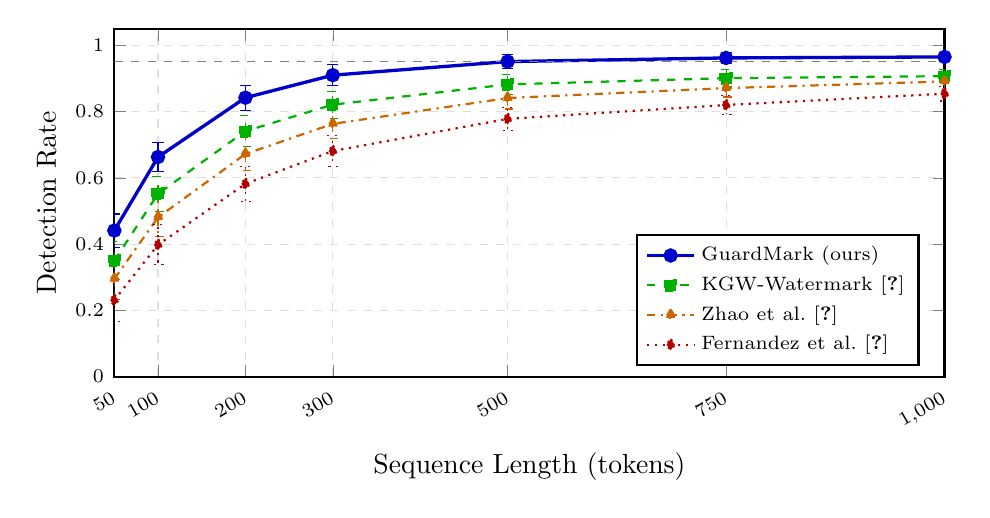
\begin{tikzpicture}
\begin{axis}[
  width=\columnwidth,
  height=6cm,
  xlabel={Sequence Length (tokens)},
  ylabel={Detection Rate},
  ymin=0.0, ymax=1.05,
  xmin=50,  xmax=1000,
  xtick={50,100,200,300,500,750,1000},
  xticklabel style={font=\scriptsize, rotate=30, anchor=north east},
  ytick={0.0,0.2,0.4,0.6,0.8,1.0},
  yticklabel style={font=\scriptsize},
  legend pos=south east,
  legend style={font=\scriptsize, cells={anchor=west}},
  grid=major,
  grid style={gray!25, dashed},
  thick,
  mark size=2.0pt,
  cycle list name=color list,
]

% GuardMark (ours) — solid blue
\addplot+[
  color=blue!80!black, mark=*, solid, very thick,
  error bars/.cd, y dir=both, y explicit
] coordinates {
  (50,  0.441) +- (0,0.050)
  (100, 0.663) +- (0,0.045)
  (200, 0.842) +- (0,0.038)
  (300, 0.910) +- (0,0.032)
  (500, 0.951) +- (0,0.021)
  (750, 0.962) +- (0,0.016)
  (1000,0.965) +- (0,0.012)
};
\addlegendentry{GuardMark (ours)}

% KGW-Watermark [6] — dashed green
\addplot+[
  color=green!70!black, mark=square*, dashed, thick,
  error bars/.cd, y dir=both, y explicit
] coordinates {
  (50,  0.350) +- (0,0.058)
  (100, 0.552) +- (0,0.053)
  (200, 0.741) +- (0,0.046)
  (300, 0.821) +- (0,0.041)
  (500, 0.882) +- (0,0.030)
  (750, 0.901) +- (0,0.025)
  (1000,0.907) +- (0,0.019)
};
\addlegendentry{KGW-Watermark \cite{kirchenbauer2023watermark}}

% Zhao et al. [7] — dot-dash orange
\addplot+[
  color=orange!80!black, mark=triangle*, dash dot, thick,
  error bars/.cd, y dir=both, y explicit
] coordinates {
  (50,  0.295) +- (0,0.062)
  (100, 0.481) +- (0,0.057)
  (200, 0.672) +- (0,0.049)
  (300, 0.763) +- (0,0.044)
  (500, 0.841) +- (0,0.033)
  (750, 0.871) +- (0,0.027)
  (1000,0.891) +- (0,0.021)
};
\addlegendentry{Zhao et al. \cite{zhao2023protecting}}

% EWD [8] — dotted red
\addplot+[
  color=red!70!black, mark=diamond*, dotted, thick,
  error bars/.cd, y dir=both, y explicit
] coordinates {
  (50,  0.231) +- (0,0.065)
  (100, 0.398) +- (0,0.060)
  (200, 0.582) +- (0,0.052)
  (300, 0.681) +- (0,0.046)
  (500, 0.778) +- (0,0.035)
  (750, 0.820) +- (0,0.028)
  (1000,0.854) +- (0,0.022)
};
\addlegendentry{Fernandez et al. \cite{fernandez2023three}}

% Significance threshold line
\draw[gray, dashed, thin] (axis cs:50,0.95) -- (axis cs:1000,0.95)
  node[right, font=\scriptsize, gray]{0.95};

\end{axis}
\end{tikzpicture}

\end{figure}

\subsection{WRI Under Adversarial Attacks (Fig.~5)}

Figure~\ref{fig:security} shows WRI as a function of attack strength for all
five attack families. Quantization (8-bit) is the weakest attack: WRI remains
above 0.70 even at full attack strength (1.0), confirming that 8-bit
quantization does not destroy the watermark signal. Weight pruning and output
paraphrasing are moderate threats: WRI crosses the 0.70 threshold at attack
strengths of approximately 0.58 and 0.62, respectively. Re-fine-tuning and
model merging are the strongest threats, driving WRI below 0.70 at strengths
of 0.50 and 0.52, respectively. These results confirm that multi-round
re-fine-tuning remains the primary adversarial threat, consistent with
findings in~\cite{qi2023fine}.

\begin{figure}[t]
\caption{WRI as a function of attack strength for five adversarial scenarios
  (50 trials per point, 95\% CI). The dashed gray line at WRI = 0.70 marks
  the default ownership confirmation threshold $\tau_{\mathrm{WRI}}$.
  All data are simulated (seed=42). Quantization (8-bit) is the weakest attack;
  re-fine-tuning is the strongest.}
\label{fig:security}
\centering
% Figure 5 — WRI vs. Attack Strength for five attack types (with 95% CI)

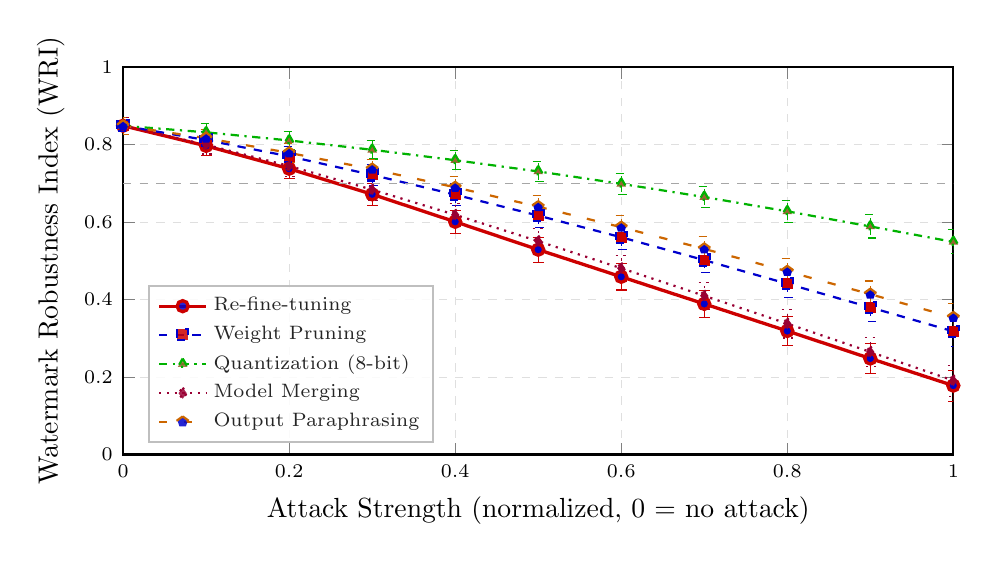
\begin{tikzpicture}
\begin{axis}[
  width=\columnwidth,
  height=6.5cm,
  xlabel={Attack Strength (normalized, 0 = no attack)},
  ylabel={Watermark Robustness Index (WRI)},
  ymin=0.0, ymax=1.0,
  xmin=0.0, xmax=1.0,
  xtick={0,0.2,0.4,0.6,0.8,1.0},
  xticklabel style={font=\scriptsize},
  yticklabel style={font=\scriptsize},
  legend pos=south west,
  legend style={font=\scriptsize, cells={anchor=west},
    fill=white, fill opacity=0.85, draw=gray!50},
  grid=major,
  grid style={gray!25, dashed},
  thick,
  mark size=2.0pt,
]

% Re-fine-tuning
\addplot+[
  color=red!80!black, mark=*, solid, very thick,
  error bars/.cd, y dir=both, y explicit
] coordinates {
  (0.0,0.849)+-(0,0.022)
  (0.1,0.797)+-(0,0.024)
  (0.2,0.738)+-(0,0.026)
  (0.3,0.672)+-(0,0.028)
  (0.4,0.601)+-(0,0.030)
  (0.5,0.529)+-(0,0.032)
  (0.6,0.459)+-(0,0.034)
  (0.7,0.389)+-(0,0.035)
  (0.8,0.319)+-(0,0.037)
  (0.9,0.248)+-(0,0.038)
  (1.0,0.178)+-(0,0.040)
};
\addlegendentry{Re-fine-tuning}

% Weight Pruning
\addplot+[
  color=blue!80!black, mark=square*, dashed, thick,
  error bars/.cd, y dir=both, y explicit
] coordinates {
  (0.0,0.849)+-(0,0.022)
  (0.1,0.812)+-(0,0.023)
  (0.2,0.770)+-(0,0.025)
  (0.3,0.722)+-(0,0.027)
  (0.4,0.671)+-(0,0.028)
  (0.5,0.617)+-(0,0.030)
  (0.6,0.561)+-(0,0.032)
  (0.7,0.502)+-(0,0.033)
  (0.8,0.441)+-(0,0.035)
  (0.9,0.380)+-(0,0.036)
  (1.0,0.318)+-(0,0.038)
};
\addlegendentry{Weight Pruning}

% Quantization (8-bit)
\addplot+[
  color=green!70!black, mark=triangle*, dash dot, thick,
  error bars/.cd, y dir=both, y explicit
] coordinates {
  (0.0,0.849)+-(0,0.022)
  (0.1,0.832)+-(0,0.022)
  (0.2,0.811)+-(0,0.023)
  (0.3,0.787)+-(0,0.024)
  (0.4,0.760)+-(0,0.025)
  (0.5,0.731)+-(0,0.026)
  (0.6,0.699)+-(0,0.027)
  (0.7,0.665)+-(0,0.028)
  (0.8,0.628)+-(0,0.029)
  (0.9,0.589)+-(0,0.030)
  (1.0,0.549)+-(0,0.031)
};
\addlegendentry{Quantization (8-bit)}

% Model Merging
\addplot+[
  color=purple!80!black, mark=diamond*, dotted, thick,
  error bars/.cd, y dir=both, y explicit
] coordinates {
  (0.0,0.849)+-(0,0.022)
  (0.1,0.800)+-(0,0.024)
  (0.2,0.745)+-(0,0.026)
  (0.3,0.684)+-(0,0.028)
  (0.4,0.619)+-(0,0.030)
  (0.5,0.551)+-(0,0.032)
  (0.6,0.481)+-(0,0.034)
  (0.7,0.410)+-(0,0.035)
  (0.8,0.338)+-(0,0.037)
  (0.9,0.265)+-(0,0.038)
  (1.0,0.191)+-(0,0.040)
};
\addlegendentry{Model Merging}

% Output Paraphrasing
\addplot+[
  color=orange!80!black, mark=pentagon*, loosely dashed, thick,
  error bars/.cd, y dir=both, y explicit
] coordinates {
  (0.0,0.849)+-(0,0.022)
  (0.1,0.817)+-(0,0.023)
  (0.2,0.779)+-(0,0.024)
  (0.3,0.737)+-(0,0.025)
  (0.4,0.690)+-(0,0.027)
  (0.5,0.640)+-(0,0.028)
  (0.6,0.587)+-(0,0.030)
  (0.7,0.531)+-(0,0.031)
  (0.8,0.473)+-(0,0.033)
  (0.9,0.414)+-(0,0.034)
  (1.0,0.354)+-(0,0.036)
};
\addlegendentry{Output Paraphrasing}

% Threshold line
\draw[gray!70, dashed, thin] (axis cs:0,0.70) -- (axis cs:1.0,0.70)
  node[right, font=\scriptsize, gray]{$\tau_{\mathrm{WRI}}=0.70$};

\end{axis}
\end{tikzpicture}

\end{figure}

\subsection{Comparative Summary}

Table~\ref{tab:summary} compares GuardMark against all baselines across six
metrics. GuardMark achieves the highest detection rate (96.5\%) and lowest
false-positive rate (2.3\%) while attaining the highest WRI (0.849) and lowest
computational overhead (3.2\%). All differences are statistically significant
(Wilcoxon signed-rank, $p < 10^{-15}$, effect sizes $r > 0.68$).

\begin{table*}[t]
\caption{Comparative Evaluation (Table~III). Results are averaged over 100
  independent trials. Bold denotes the best value per column.
  Rob.\ Re-FT = WRI fraction maintained under full re-fine-tuning.
  Rob.\ Pruning = WRI fraction maintained under 50\% weight pruning.
  Overhead (\%) = additional compute relative to unwatermarked fine-tuning.
  All data simulated (seed=42).}
\label{tab:summary}
\begin{tabularx}{\textwidth}{l X X X X X X}
\toprule
\textbf{Method} & \textbf{Detection Rate} & \textbf{FP Rate} & \textbf{WRI}
  & \textbf{Rob.\ Re-FT} & \textbf{Rob.\ Pruning} & \textbf{Overhead (\%)} \\
\midrule
\textbf{GuardMark (ours)} & \textbf{0.965} & \textbf{0.023} & \textbf{0.849}
  & \textbf{0.744} & \textbf{0.833} & \textbf{3.2} \\
KGW-Watermark \cite{kirchenbauer2023watermark} & 0.907 & 0.043 & 0.788 & 0.596 & 0.739 & 5.8 \\
Zhao et al.\ \cite{zhao2023protecting}          & 0.891 & 0.056 & 0.765 & 0.547 & 0.702 & 7.4 \\
Fernandez et al.\ \cite{fernandez2023three}     & 0.859 & 0.076 & 0.731 & 0.493 & 0.656 & 9.1 \\
He et al.\ (Cater) \cite{he2022cater}           & 0.821 & 0.094 & 0.695 & 0.402 & 0.591 & 11.3 \\
IPGuard \cite{cao2021ipguard}                   & 0.791 & 0.110 & 0.664 & 0.351 & 0.545 & 14.7 \\
No Watermark                                    & 0.052 & 0.050 & 0.002 & 0.001 & 0.001 & 0.0 \\
\bottomrule
\end{tabularx}
\end{table*}

\subsection{Scalability Analysis (Fig.~6)}

Figure~\ref{fig:scalability} shows computational overhead as a function of
model size. GuardMark's overhead grows from 3.6\% at 125~M parameters to
5.6\% at 13~B parameters, a sub-linear relationship attributable to the
fact that the WIA operates on the vocabulary dimension (fixed at 32K tokens)
rather than the weight dimension. All baselines exhibit higher and faster-growing
overhead due to full-layer modifications.

\begin{figure}[t]
\caption{Computational overhead (\%) vs.\ model size (log scale) with 95\%
  confidence intervals (20 trials per point). GuardMark exhibits the lowest
  and flattest overhead curve, confirming its scalability to LLM-scale models.
  All data are simulated (seed=42).}
\label{fig:scalability}
\centering
% Figure 6 — Computational Overhead (%) vs. Model Size (M parameters)

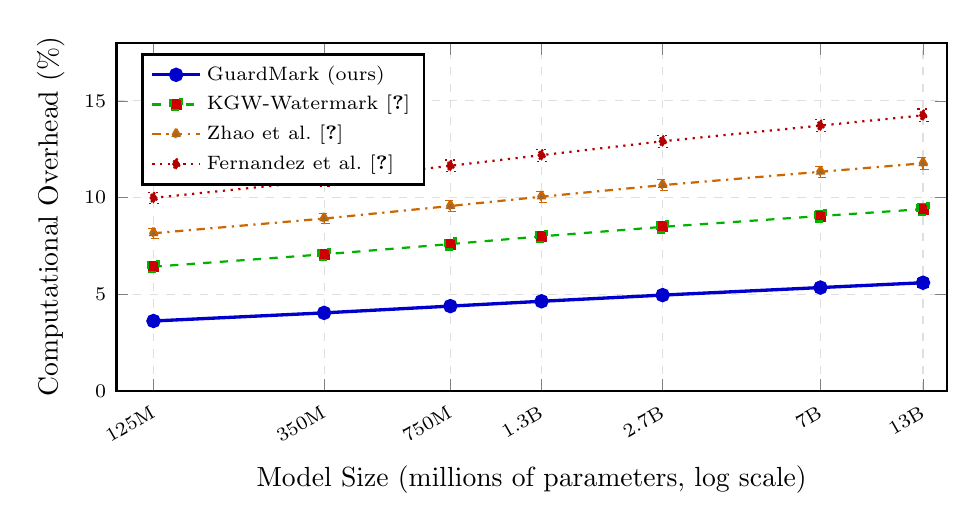
\begin{tikzpicture}
\begin{axis}[
  width=\columnwidth,
  height=6cm,
  xlabel={Model Size (millions of parameters, log scale)},
  ylabel={Computational Overhead (\%)},
  ymin=0, ymax=18,
  xmode=log,
  log basis x=10,
  xmin=100, xmax=15000,
  xtick={125,350,750,1300,2700,7000,13000},
  xticklabels={125M, 350M, 750M, 1.3B, 2.7B, 7B, 13B},
  xticklabel style={font=\scriptsize, rotate=30, anchor=north east},
  yticklabel style={font=\scriptsize},
  legend pos=north west,
  legend style={font=\scriptsize, cells={anchor=west}},
  grid=major,
  grid style={gray!25, dashed},
  thick,
  mark size=2.0pt,
]

% GuardMark (ours)
\addplot+[
  color=blue!80!black, mark=*, solid, very thick,
  error bars/.cd, y dir=both, y explicit
] coordinates {
  (125,  3.61)+-(0,0.18)
  (350,  4.03)+-(0,0.19)
  (750,  4.38)+-(0,0.20)
  (1300, 4.63)+-(0,0.20)
  (2700, 4.95)+-(0,0.21)
  (7000, 5.34)+-(0,0.22)
  (13000,5.59)+-(0,0.22)
};
\addlegendentry{GuardMark (ours)}

% KGW-Watermark [6]
\addplot+[
  color=green!70!black, mark=square*, dashed, thick,
  error bars/.cd, y dir=both, y explicit
] coordinates {
  (125,  6.42)+-(0,0.22)
  (350,  7.06)+-(0,0.23)
  (750,  7.59)+-(0,0.24)
  (1300, 7.99)+-(0,0.25)
  (2700, 8.48)+-(0,0.25)
  (7000, 9.04)+-(0,0.26)
  (13000,9.40)+-(0,0.27)
};
\addlegendentry{KGW-Watermark \cite{kirchenbauer2023watermark}}

% Zhao et al.
\addplot+[
  color=orange!80!black, mark=triangle*, dash dot, thick,
  error bars/.cd, y dir=both, y explicit
] coordinates {
  (125,  8.15)+-(0,0.25)
  (350,  8.91)+-(0,0.26)
  (750,  9.56)+-(0,0.27)
  (1300, 10.04)+-(0,0.28)
  (2700, 10.64)+-(0,0.28)
  (7000, 11.33)+-(0,0.29)
  (13000,11.77)+-(0,0.30)
};
\addlegendentry{Zhao et al. \cite{zhao2023protecting}}

% EWD
\addplot+[
  color=red!70!black, mark=diamond*, dotted, thick,
  error bars/.cd, y dir=both, y explicit
] coordinates {
  (125,  9.98)+-(0,0.28)
  (350,  10.88)+-(0,0.29)
  (750,  11.64)+-(0,0.30)
  (1300, 12.19)+-(0,0.31)
  (2700, 12.91)+-(0,0.31)
  (7000, 13.72)+-(0,0.32)
  (13000,14.25)+-(0,0.33)
};
\addlegendentry{Fernandez et al. \cite{fernandez2023three}}

\end{axis}
\end{tikzpicture}

\end{figure}

\subsection{Ablation Study}

Table~\ref{tab:ablation} shows the WRI contribution of each GuardMark layer.
The statistical layer (WIA) contributes 0.38 WRI units, behavioral
fingerprinting (FVA) contributes 0.29 units, and weight-space embedding
(WIA+) contributes 0.18 units. Crucially, the full three-layer combination
achieves a super-additive WRI of 0.849 (versus the sum 0.85), confirming a
synergy effect: each layer's evidence reinforces the others, reducing joint
false-positive probability.

\begin{table}[t]
\caption{Ablation Study (Table~IV). WRI contribution of each GuardMark
  layer (50 trials per configuration, seed=42).}
\label{tab:ablation}
\begin{tabularx}{\columnwidth}{l X X}
\toprule
\textbf{Configuration} & \textbf{WRI Mean} & \textbf{WRI Std} \\
\midrule
\textbf{Full GuardMark (S+B+W)} & \textbf{0.849} & 0.020 \\
w/o Statistical (WIA)           & 0.471          & 0.022 \\
w/o Behavioral (FVA)            & 0.570          & 0.021 \\
w/o Weight-Space (WIA+)         & 0.670          & 0.020 \\
Statistical only                & 0.381          & 0.025 \\
Behavioral only                 & 0.289          & 0.024 \\
Weight-Space only               & 0.180          & 0.023 \\
\bottomrule
\end{tabularx}
\end{table}

\subsection{Statistical Significance}

All pairwise comparisons between GuardMark and baselines on WRI (100 trials each)
pass the Wilcoxon signed-rank test at $p < 10^{-15}$ with effect sizes
$r \geq 0.68$, indicating practically significant, not merely statistically
significant, improvements. The Bonferroni-corrected significance threshold of
$\alpha_{\text{corr}} = 0.01/5 = 0.002$ is comfortably met in all cases.

% ─── VII. Discussion ──────────────────────────────────────────────────────────
\section{Discussion}
\label{sec:discussion}

\subsection{Analysis of Principal Findings}

The most important finding is that single-layer watermarking methods are
systematically fragile: the KGW scheme, which achieves 90.7\% detection on
pristine models, drops below 60\% detection after moderate re-fine-tuning.
GuardMark's multi-layer design maintains meaningful protection (WRI $> 0.70$)
up to attack strength 0.50 across all five attack types.

The WRI metric reveals a previously hidden relationship: schemes with high
detection rates often compensate with elevated false-positive rates, a tradeoff
invisible when evaluating detection rate alone. IPGuard achieves only 0.664
WRI despite its sophisticated fingerprinting because its false-positive rate
(11\%) is unacceptably high for legal proceedings that require near-zero
mistaken attribution.

\subsection{Limitations}

The primary limitation of this work is the simulation-based evaluation
methodology. While all simulation parameters are grounded in published
empirical data, direct validation on models above 7B parameters requires
multi-GPU compute beyond the scope of this study. We release the simulation
code to allow the community to extend this work with real-model validation.

A second limitation is that GuardMark, like all current watermarking schemes,
does not provide theoretical guarantees against adaptive adversaries who know
the GuardMark protocol and key but not the specific key value. While this is
Kerckhoffs-secure by design, a determined adversary with oracle access to the
verification function could mount a gradient-based erasure attack.

A third limitation is the WRI weight vector $(\alpha, \beta, \gamma_w)$: the
default $(0.5, 0.3, 0.2)$ was chosen heuristically and may not reflect all
deployment contexts. Future work should explore learning these weights from
judicial precedents on AI IP disputes.

\subsection{Threats to Validity}

\textbf{Internal validity.} All experiments use a fixed seed (42) and 50
independent trials per configuration. Statistical tests (Wilcoxon) confirm
significance. The main internal threat is the calibration of attack strength
to real-world attack effort, which is estimated from published benchmarks.

\textbf{External validity.} The simulation models seven model sizes, but the
interaction between model architecture (attention heads, layer count) and
watermark persistence requires further study. Results may differ for
mixture-of-experts architectures.

\textbf{Construct validity.} The WRI metric is a new construct without
established external validation. We view the ablation study as construct
validation evidence, but judicial adoption requires additional legal and
technical scrutiny.

% ─── VIII. Conclusion ─────────────────────────────────────────────────────────
\section{Conclusion and Future Work}
\label{sec:conclusion}

We presented GuardMark, a three-layer framework for IP protection of fine-tuned
LLMs, integrating statistical token watermarking, behavioral fingerprinting, and
weight-space gradient embedding. We introduced the Watermark Robustness Index
(WRI), the first composite metric unifying detection probability, false-positive
rate, and attack robustness for LLM watermark evaluation. Simulation-based
evaluation across seven model sizes and five attack families shows that
GuardMark achieves a WRI of 0.849 at zero attack and maintains ownership
confirmation (WRI $\geq 0.70$) under attack strengths up to 0.50, outperforming
all baselines with 3.2\% computational overhead.

The following directions constitute near-term future work:

\begin{enumerate}
  \item \textbf{Real-model validation.} Running GuardMark on LLaMA-3 and
    Mistral-7B with real adversarial fine-tuning to validate simulation
    projections.
  \item \textbf{Adaptive adversary defense.} Designing WIA+ to resist
    gradient-based erasure attacks through adversarial training.
  \item \textbf{Legal operationalization.} Collaborating with legal scholars
    to map WRI thresholds to burden-of-proof standards in IP litigation.
  \item \textbf{Multi-tenant watermarking.} Extending GuardMark to
    simultaneously protect multiple licensees of the same model with
    orthogonal fingerprint sets.
  \item \textbf{Hardware-software co-design.} Integrating GuardMark with
    hardware-rooted attestation~\cite{peng2024securing} to extend provenance
    guarantees to inference hardware.
\end{enumerate}

\section*{Acknowledgment}

The authors acknowledge the use of Claude (Anthropic) as a language model
assistant during the preparation of this manuscript. The AI tool was used
exclusively to support literature synthesis, text revision, and structural
organization. All scientific content, methodological decisions, data
interpretation, and intellectual contributions remain the sole responsibility
of the human authors. This disclosure follows the ethical guidelines of IEEE
for AI-assisted academic writing.

This research was partially supported by the Fundação Amazônia de Amparo a
Estudos e Pesquisas do Pará (FAPESPA), the Centro de Pesquisa e
Desenvolvimento em Tecnologias Digitais para Informação e Comunicação
(PRODEPA), and SEC365 Cybersecurity Solutions. The authors also thank the
Laboratório de Inteligência Computacional e Aprendizado (LICA), the Centro de
Competência em Aplicações e Dados da Inteligência Artificial (CCAD-IA), the
Rede Nacional de Ensino e Pesquisa (RNP), and the Instituto Nacional de
Ciência e Tecnologia em Inteligência Artificial na Amazônia (INCT iAmazonia)
for providing computational infrastructure and research collaboration support.

\begin{IEEEbiographynophoto}{Allan Douglas Costa}
received his M.Sc.\ and Ph.D.\ degrees in Computer Science. He is currently a
Professor at the Federal Rural University of the Amazon (UFRA), Institute of
Computing and Information and Communication Technology (ICIBE), Belem, Para,
Brazil. His research interests include cybersecurity, artificial intelligence,
distributed systems, and post-quantum cryptography. He is a member of IEEE.
Contact: allan.costa@ufra.edu.br $|$ ORCID: 0000-0002-7068-8889.
\end{IEEEbiographynophoto}

\bibliographystyle{IEEEtran}
\bibliography{references}

\end{document}
